\begin{frame}{Le protocole éditorial du CMS Wiki}
\begin{itemize}
    \item Un historique des modifications
    \item Une documentation des modifications
    \item Des espaces de débats ("Discussion")
    \item Des principes d'auto-évaluation et d'auto-régulation (labels, bots, etc.)
\end{itemize}

\end{frame}

\begin{frame}{Historique des modifications}
\centering
    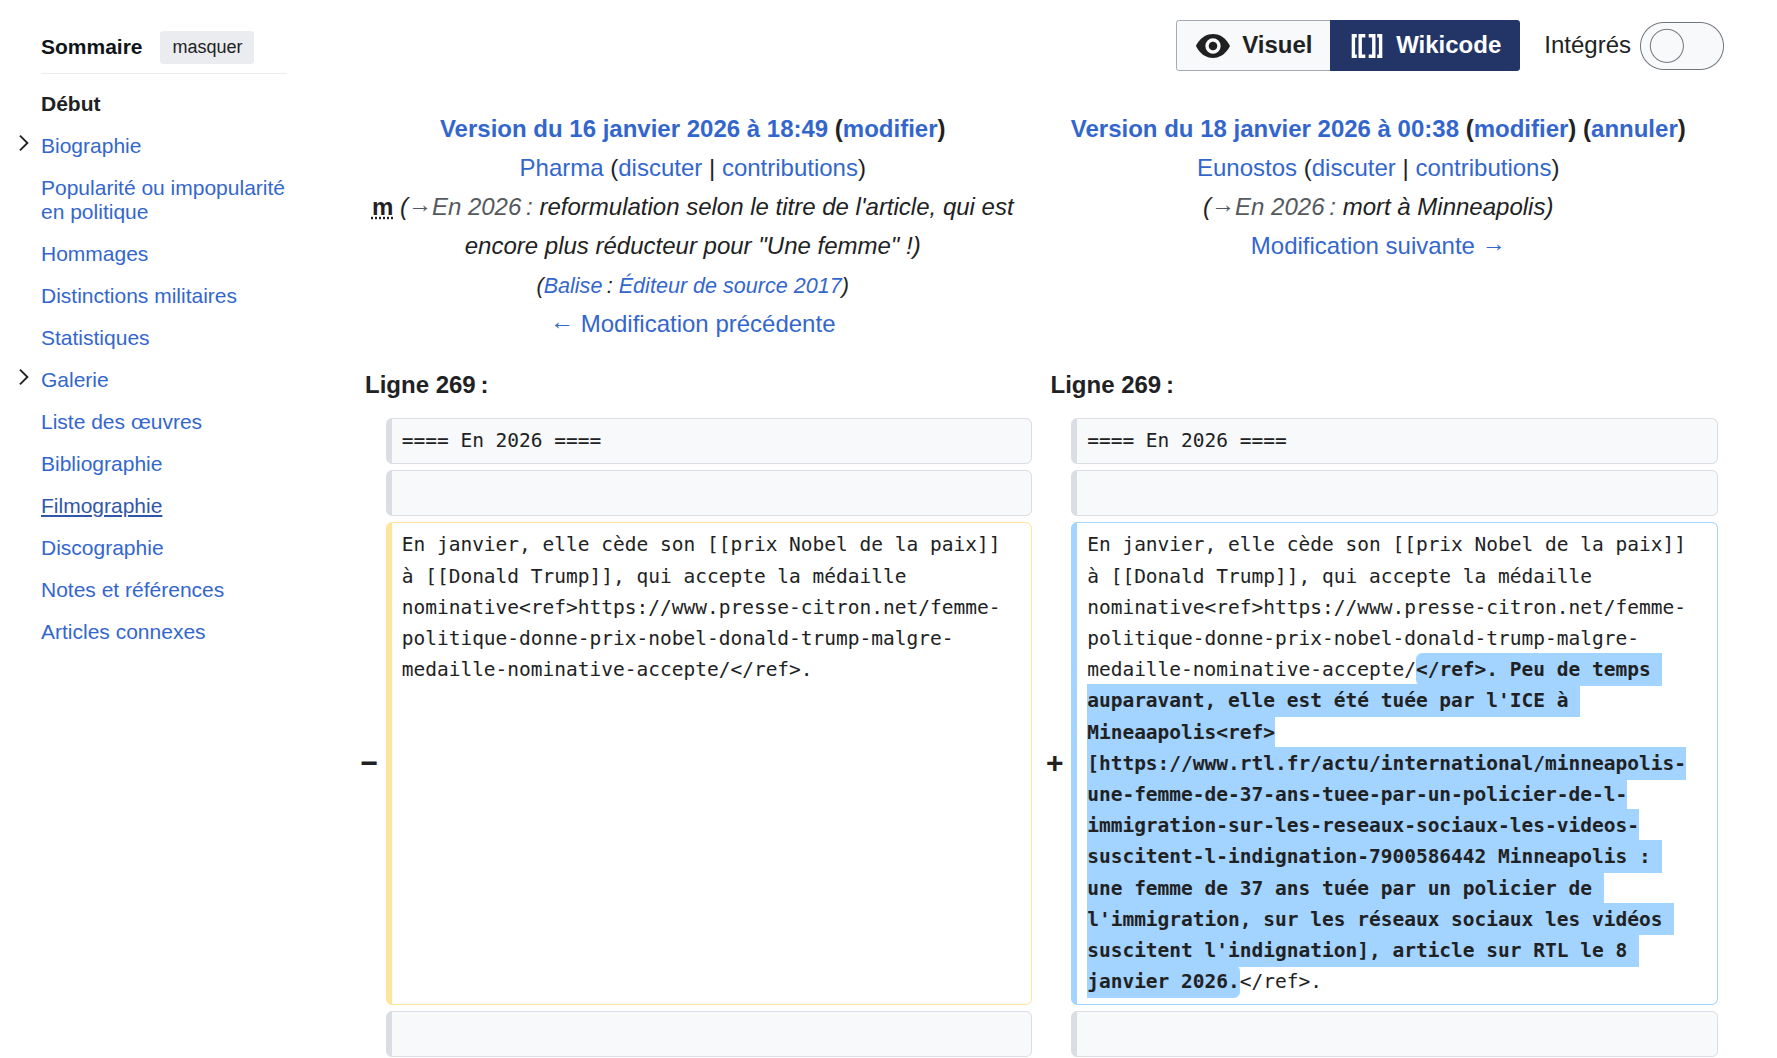
\includegraphics[width=5cm]{05_Axe1_protocoles/images/wikipedia-une-femme-dif-historique.png}
    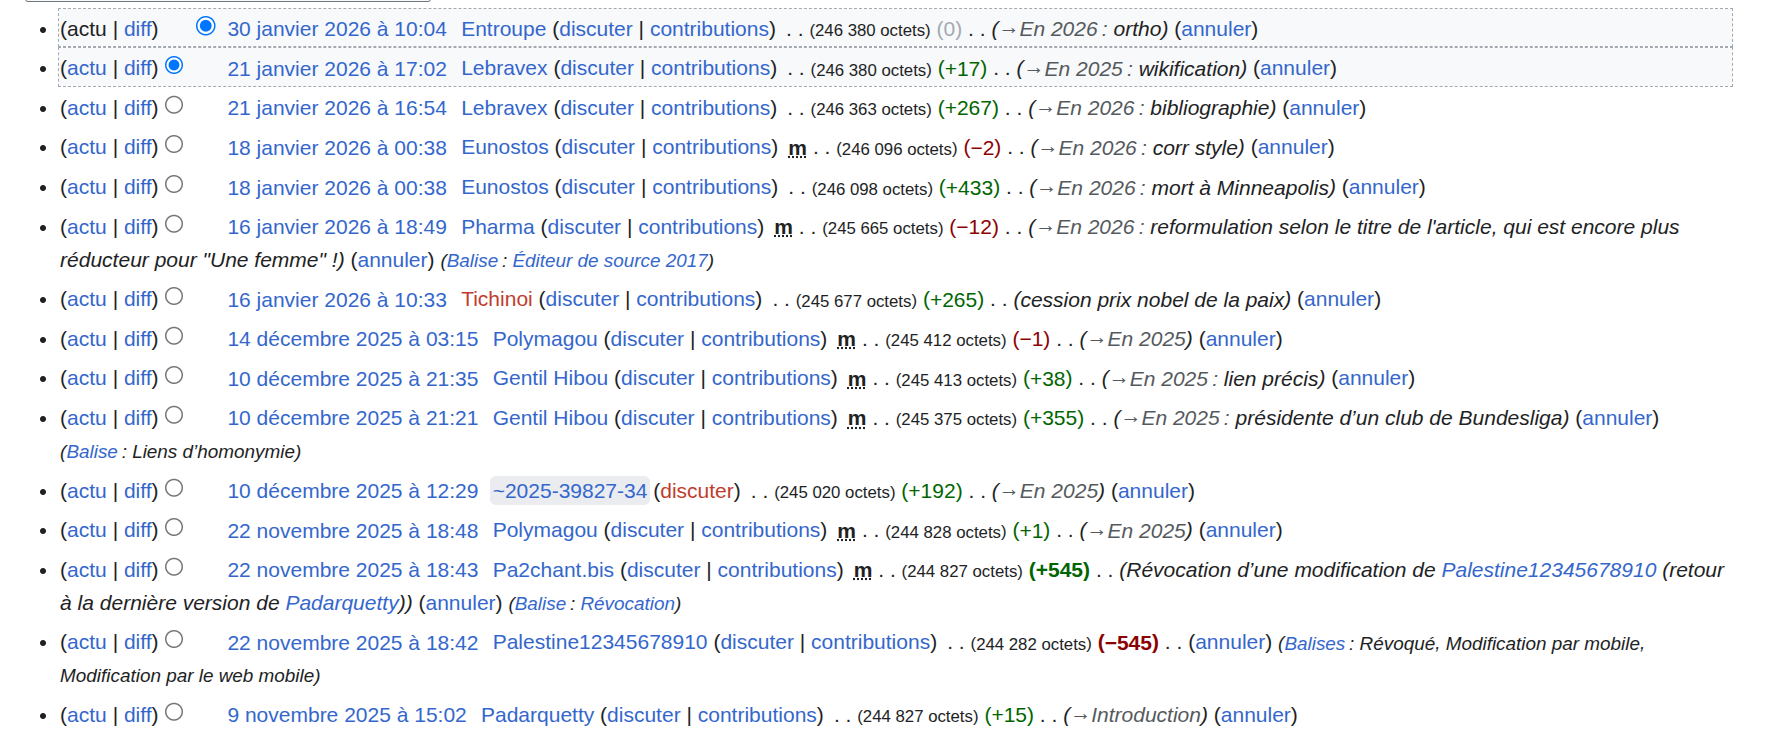
\includegraphics[width=5cm]{05_Axe1_protocoles/images/historique-une-femme.png}
\end{frame}

\begin{frame}{Documentation des modifications}
    \centering
    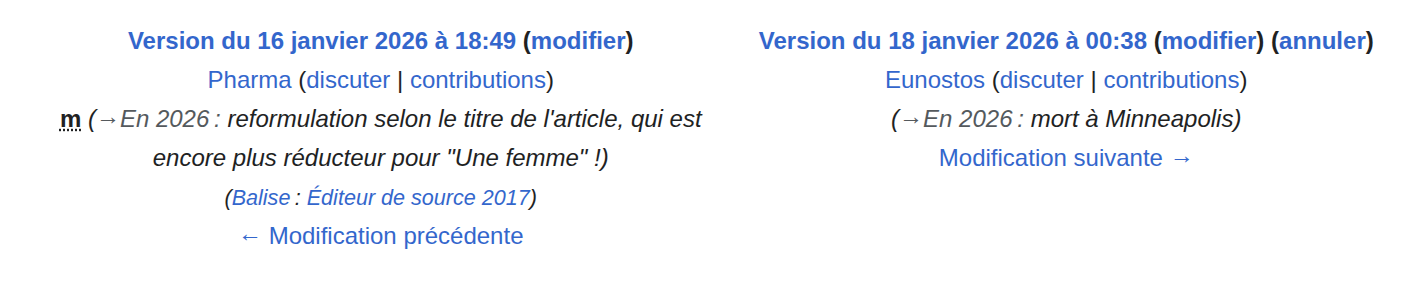
\includegraphics[width=.80\textwidth]{05_Axe1_protocoles/images/wikipedia-une-femme-commit.png}
\end{frame}

\begin{frame}{Espaces de débat}
    \centering
    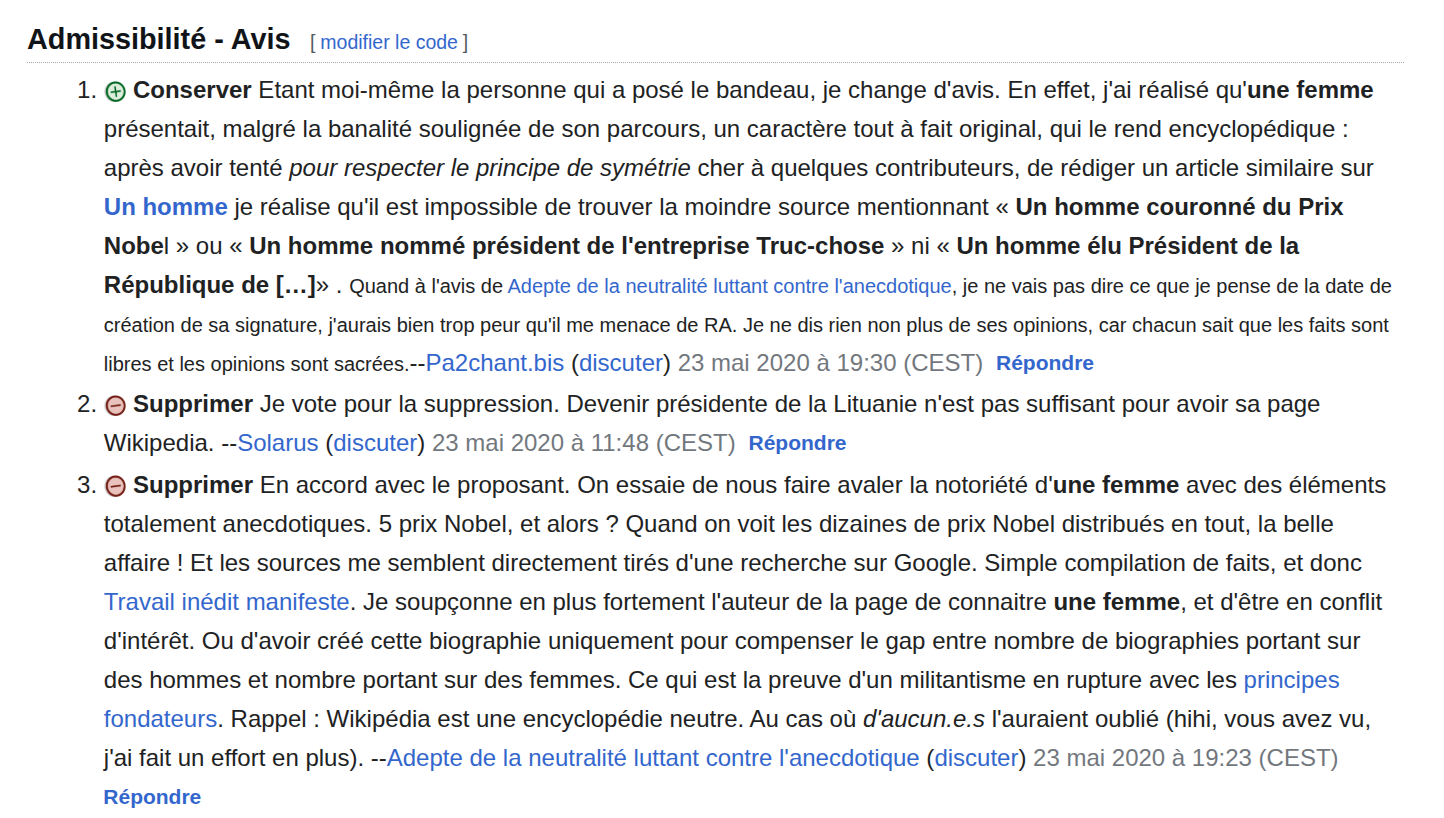
\includegraphics[width=5cm]{05_Axe1_protocoles/images/wikipedia-une-femme-admissibilite-repose.png}
    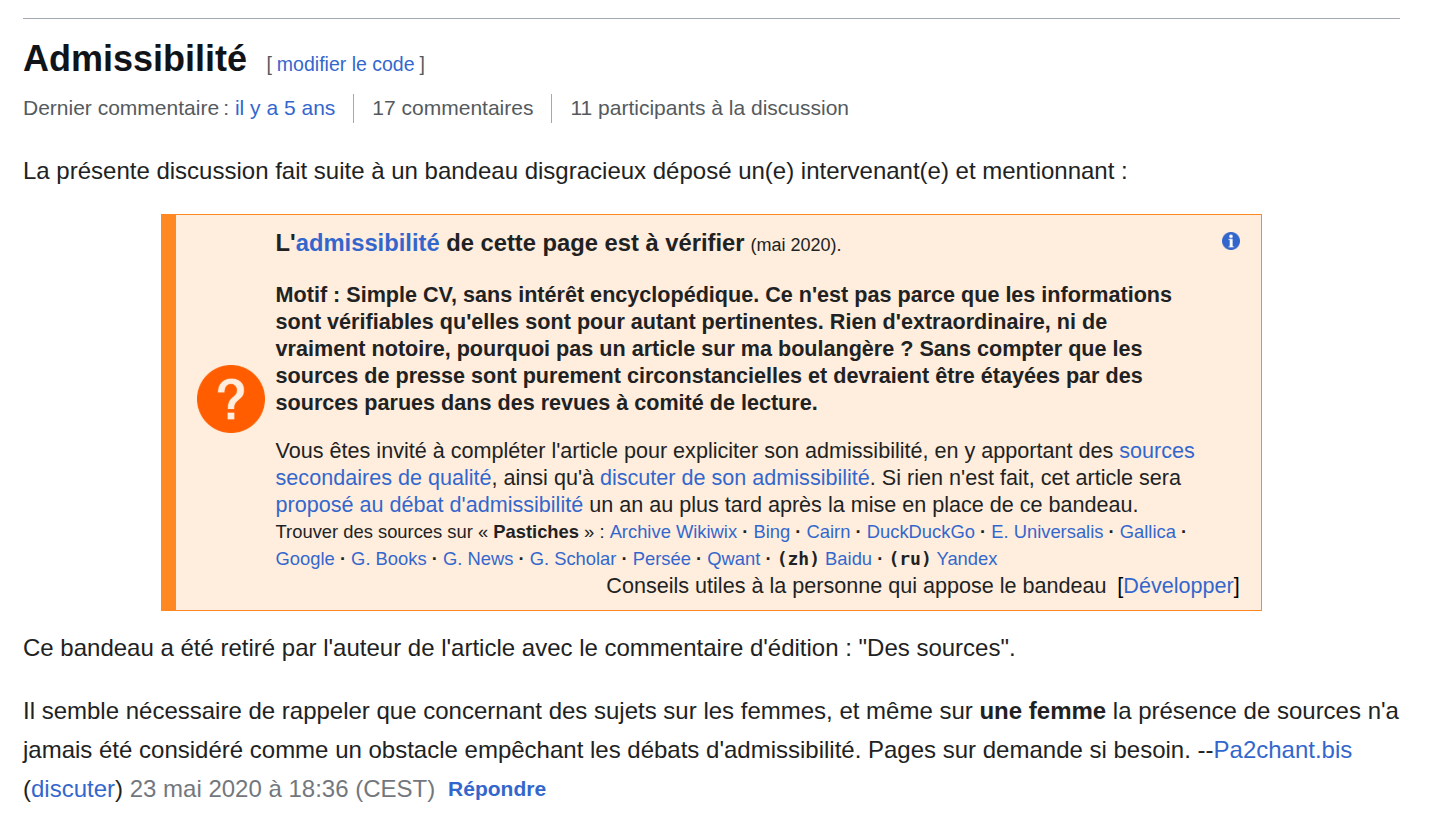
\includegraphics[width=5cm]{05_Axe1_protocoles/images/wikipedia-une-femme-admissibilite.png}
\end{frame}

\begin{frame}{Système d'auto-évaluation et d'auto-régulation}
    \centering
    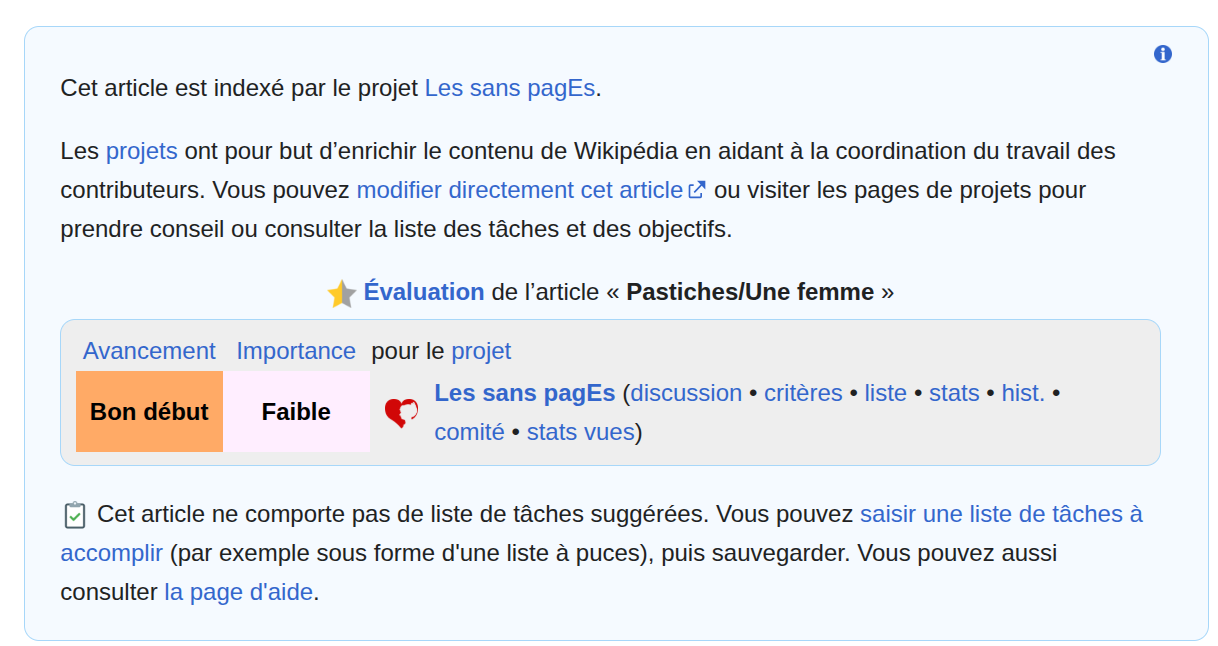
\includegraphics[width=.80\textwidth]{05_Axe1_protocoles/images/wikipedia-une-femme-auto-eval.png}
\end{frame}


\begin{frame}{Un savoir "instable", ou un savoir "éditorialisé" ?}
   \begin{itemize}
       \item Sur Wikipédia, une mise à jour constante
       \item Des contributions exponentielles
       \item Instabilité de l'encyclopédie, instabilité du savoir ?
   \end{itemize}


   \url{https://www.youtube.com/watch?v=ZOa8PAgg8ZI}


\end{frame}

\begin{frame}{Conclusion}
    La philosophie propre aux protocoles du web a participé à reconfigurer notre culture et notre manière de penser l'autorité. Ces protocoles ont encouragé l'émergence d'un nouveau modèle épistémique dont Wikipédia, incarnation de la nouvelle génération encyclopédique, peut témoigner. En passant du paradigme de l'édition à celui de l'éditorialisation, Wikipédia défend l'idée d'un savoir processuel, instable, sans cesse en construction. Un savoir qui, par ailleurs, doit se négocier au sein de d'une communauté - redéfinissant en cela notre conception même de l'autorité, sur laquelle s'était fondé le système éditorial moderne.
\end{frame}

\begin{frame}{Atelier: écrire, éditer sur un Wiki}
    \centering
    
\includegraphics[width=5cm]{05_Axe1_protocoles/images/qr-code-atelier-wiki.png}
\end{frame}